\documentclass[12pt]{article} % use larger type; default would be 10pt
\usepackage[utf8]{inputenc}
\usepackage{geometry} % to change the page dimensions
\geometry{letterpaper} 
\geometry{letterpaper} % or letterpaper (US) or a5paper or....
% \geometry{margin=2in} % for example, change the margins to 2 inches all round
% \geometry{landscape} % set up the page for landscape
%   read geometry.pdf for detailed page layout information
\usepackage{graphicx} % support the \includegraphics command 
\usepackage{booktabs} % for much better looking tables
\usepackage{array} % for arrays
\usepackage{verbatim} % adds environment for commenting out blocks of text
\usepackage{eqnarray, amsmath}
\usepackage[makeroom]{cancel}
\usepackage{sidecap}
\usepackage[ngerman]{babel}
\usepackage[utf8]{inputenc}
\usepackage{pgfplots}
\pgfplotsset{compat=1.14}
\usetikzlibrary{positioning}
\usepackage{siunitx}
\usepackage{fancyhdr} % This should be set AFTER setting up the page geometry
\pagestyle{fancy} % options: empty , plain , fancy
\renewcommand{\headrulewidth}{0pt} % customise the layout...
\lhead{}\chead{}\rhead{}
\lfoot{}\cfoot{\thepage}\rfoot{}
%%% SECTION TITLE APPEARANCE
\usepackage{sectsty}
\allsectionsfont{\sffamily\mdseries\upshape} % (See the fntguide.pdf for font help)
% (This matches ConTeXt defaults)
%%% ToC (table of contents) APPEARANCE
\usepackage[nottoc,notlof,notlot]{tocbibind} % Put the bibliography in the ToC
\usepackage[titles,subfigure]{tocloft} % Alter the style of the Table of Contents
\usepackage[colorlinks=true,citecolor=black,linkcolor=black,urlcolor=blue]{hyperref}
\usepackage{subcaption}
\renewcommand{\cftsecfont}{\rmfamily\mdseries\upshape}
\renewcommand{\cftsecpagefont}{\rmfamily\mdseries\upshape} % No bold!
\usepackage{pdfpages}
%\includepdf[pages={1}]{myfile.pdf}
\usepackage{listings}
\usepackage{color} %red, green, blue, yellow, cyan, magenta, black, white
\definecolor{mygreen}{RGB}{28,172,0} % color values Red, Green, Blue
\definecolor{mylilas}{RGB}{170,55,241}




\title{{\bf{Project 2}}}
\author{Abraham Jacob Reines}
\date{May 5, 2022} % Activate to display a given date or no date (if empty),
         % otherwise the current date is printed 
\begin{document}
\maketitle
\hfill
\newpage

\section{Project 4: Chaos in Newton’s Method}
  \subsection{Applying Newton’s Method for 'Part a'}\par
  The task is to apply Newton’s Method to   
  \begin{equation}\label{eqn}  f(x) = x(x - 1)(x + \frac{1}{2})  \end{equation}
  for many  initial guesses on (-2,2), and plot the zero it converges to as a function of the initial point.  This is accomplished using 'AChaoticNewton.m' function and on lines 1 through 29 of 'Project2.m' algorithm.  The figure below illustrates even
as you make the interval smaller, the jumpiness of the solution looks similar.  This means we have a self-similar, or chaotic behavior.\par
The solution procedure accesses the Newton function written to find roots.  The algorithm plots the 'Number found' v. 'Estimates' for Equation (1).

\begin{figure}[ht!]
    \centering
    \begin{subfigure}{0.4\textwidth}
        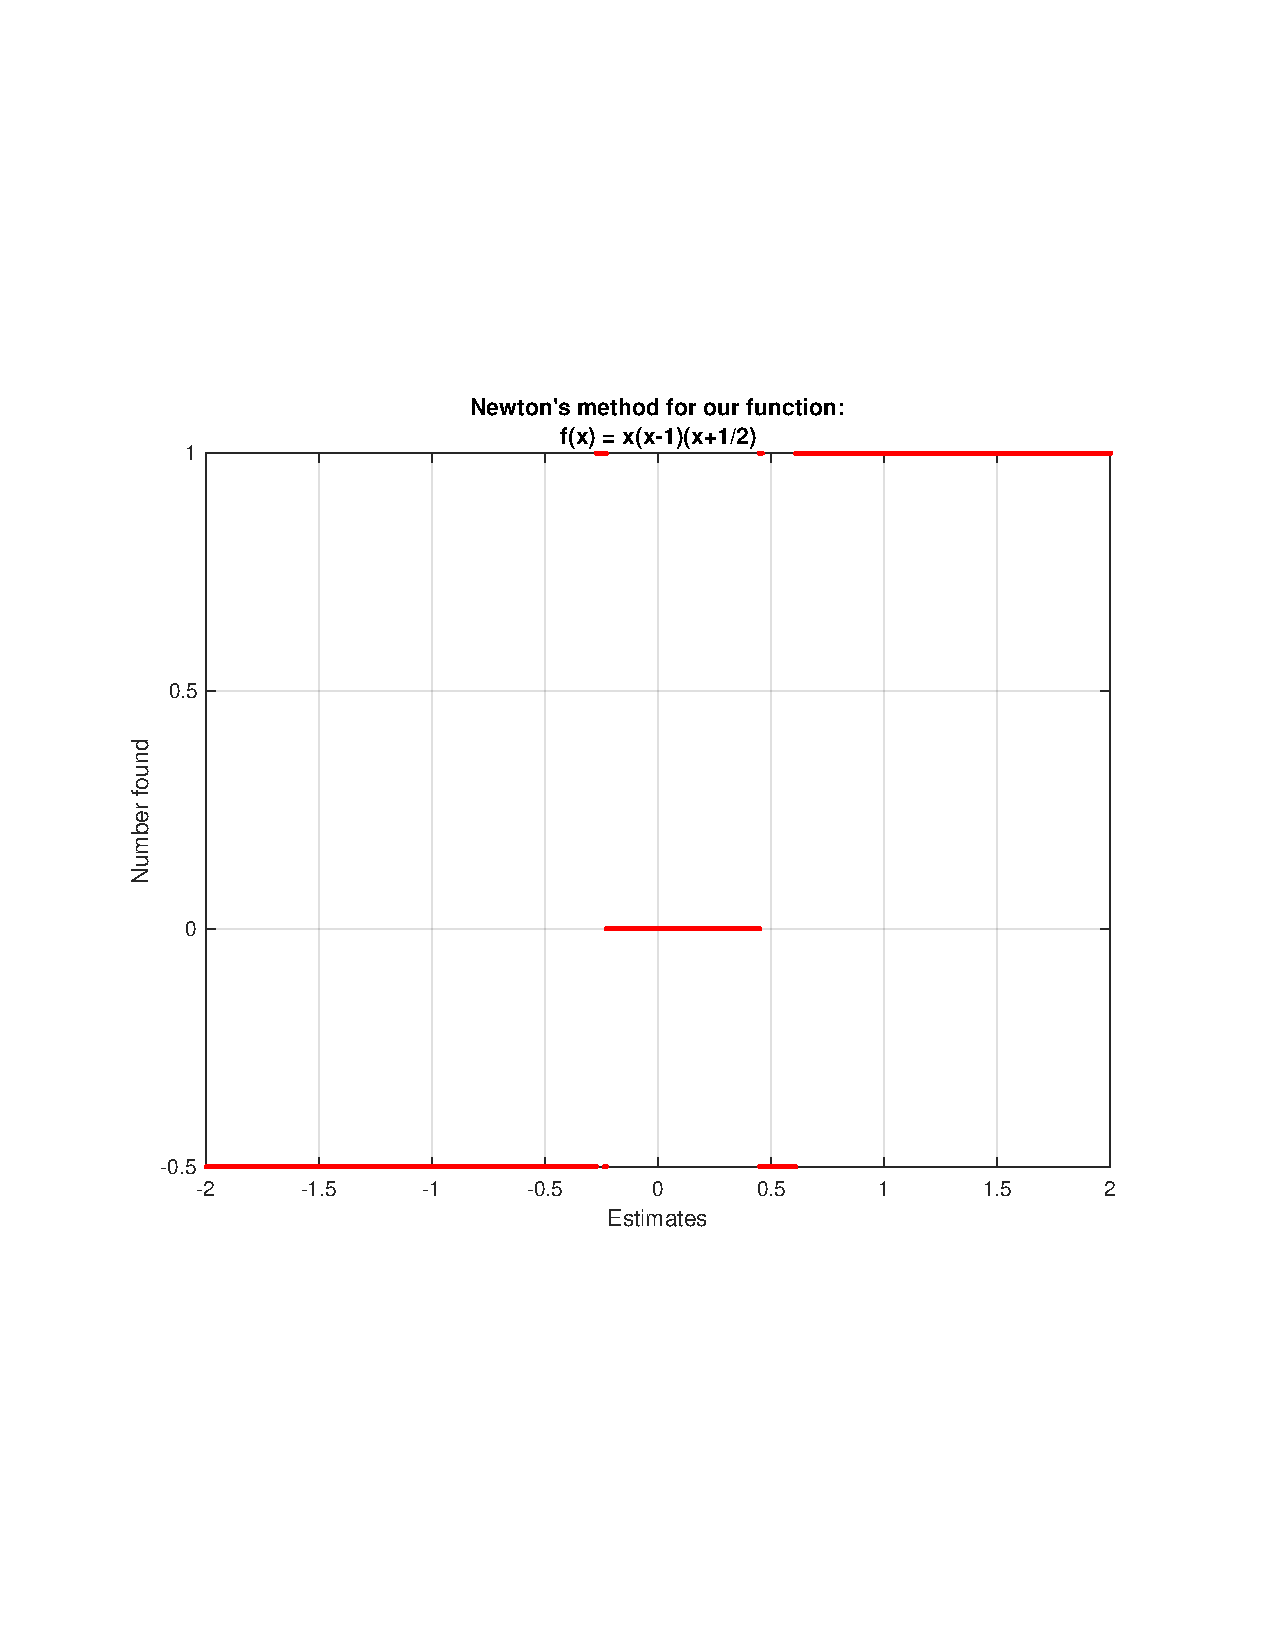
\includegraphics[width=\textwidth]{fig0.pdf}
        \caption{\small}
        \label{}
    \end{subfigure}
    \begin{subfigure}{0.4\textwidth}
        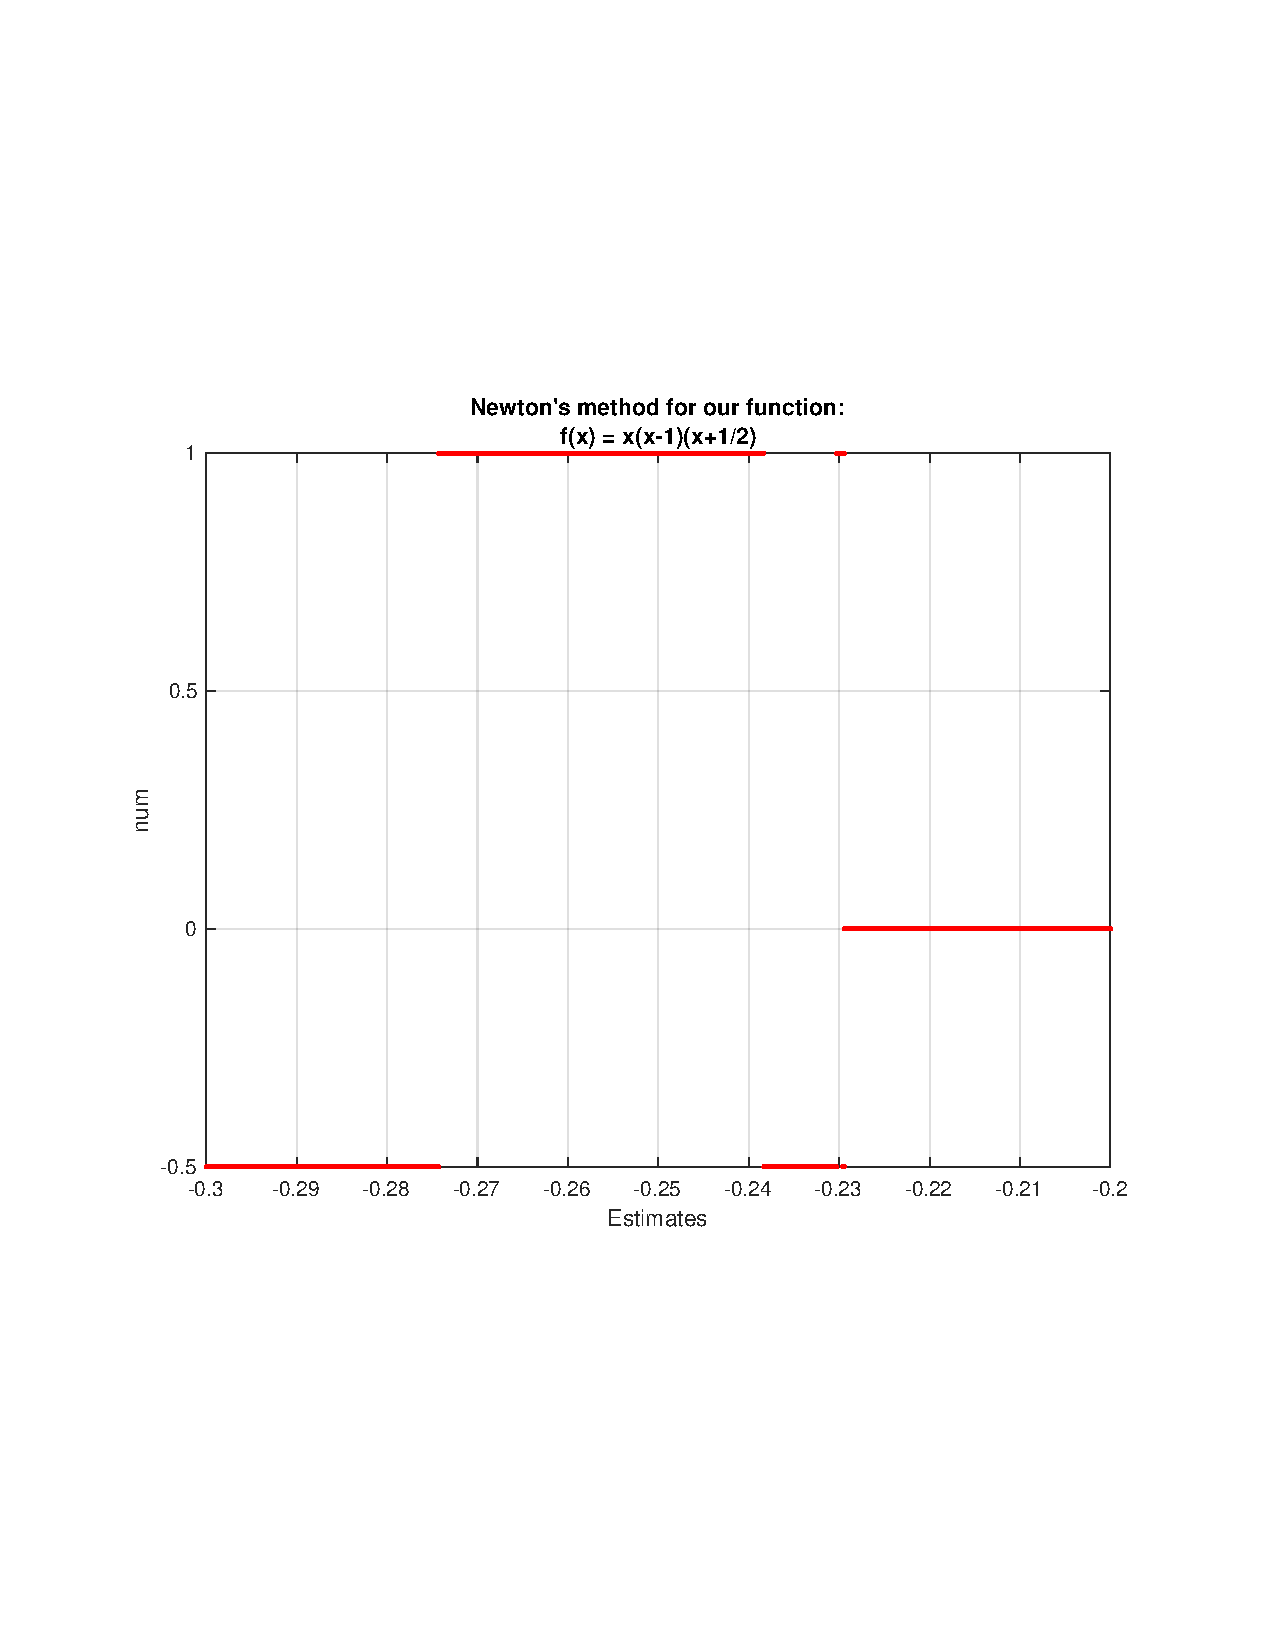
\includegraphics[width=\textwidth]{fig1.pdf}
        \caption{\small }
        \label{}
    \end{subfigure}
\end{figure}

  \hfill\newpage
  \subsection{Applying Newton's Method for 'Part b'}
  The task is to apply Newton's Method to 
  \begin{equation}\label{eqn} f(x) = x\textsuperscript{3} - 1 \end{equation}
  with initial guess a selection of complex numbers with real and imaginary parts varying from -2 to 2. After accomplishing this in lines 31 to 57 of 'Project2.m' we plotted; the plot is colored based upon which of the three roots you converge to.\par
  The solution procedure for this function requires a nested loop to compute the real and imaginary parts.  We plot the 'real' v. 'imaginary' results in a colorful figure.  See figure on next page...
  
        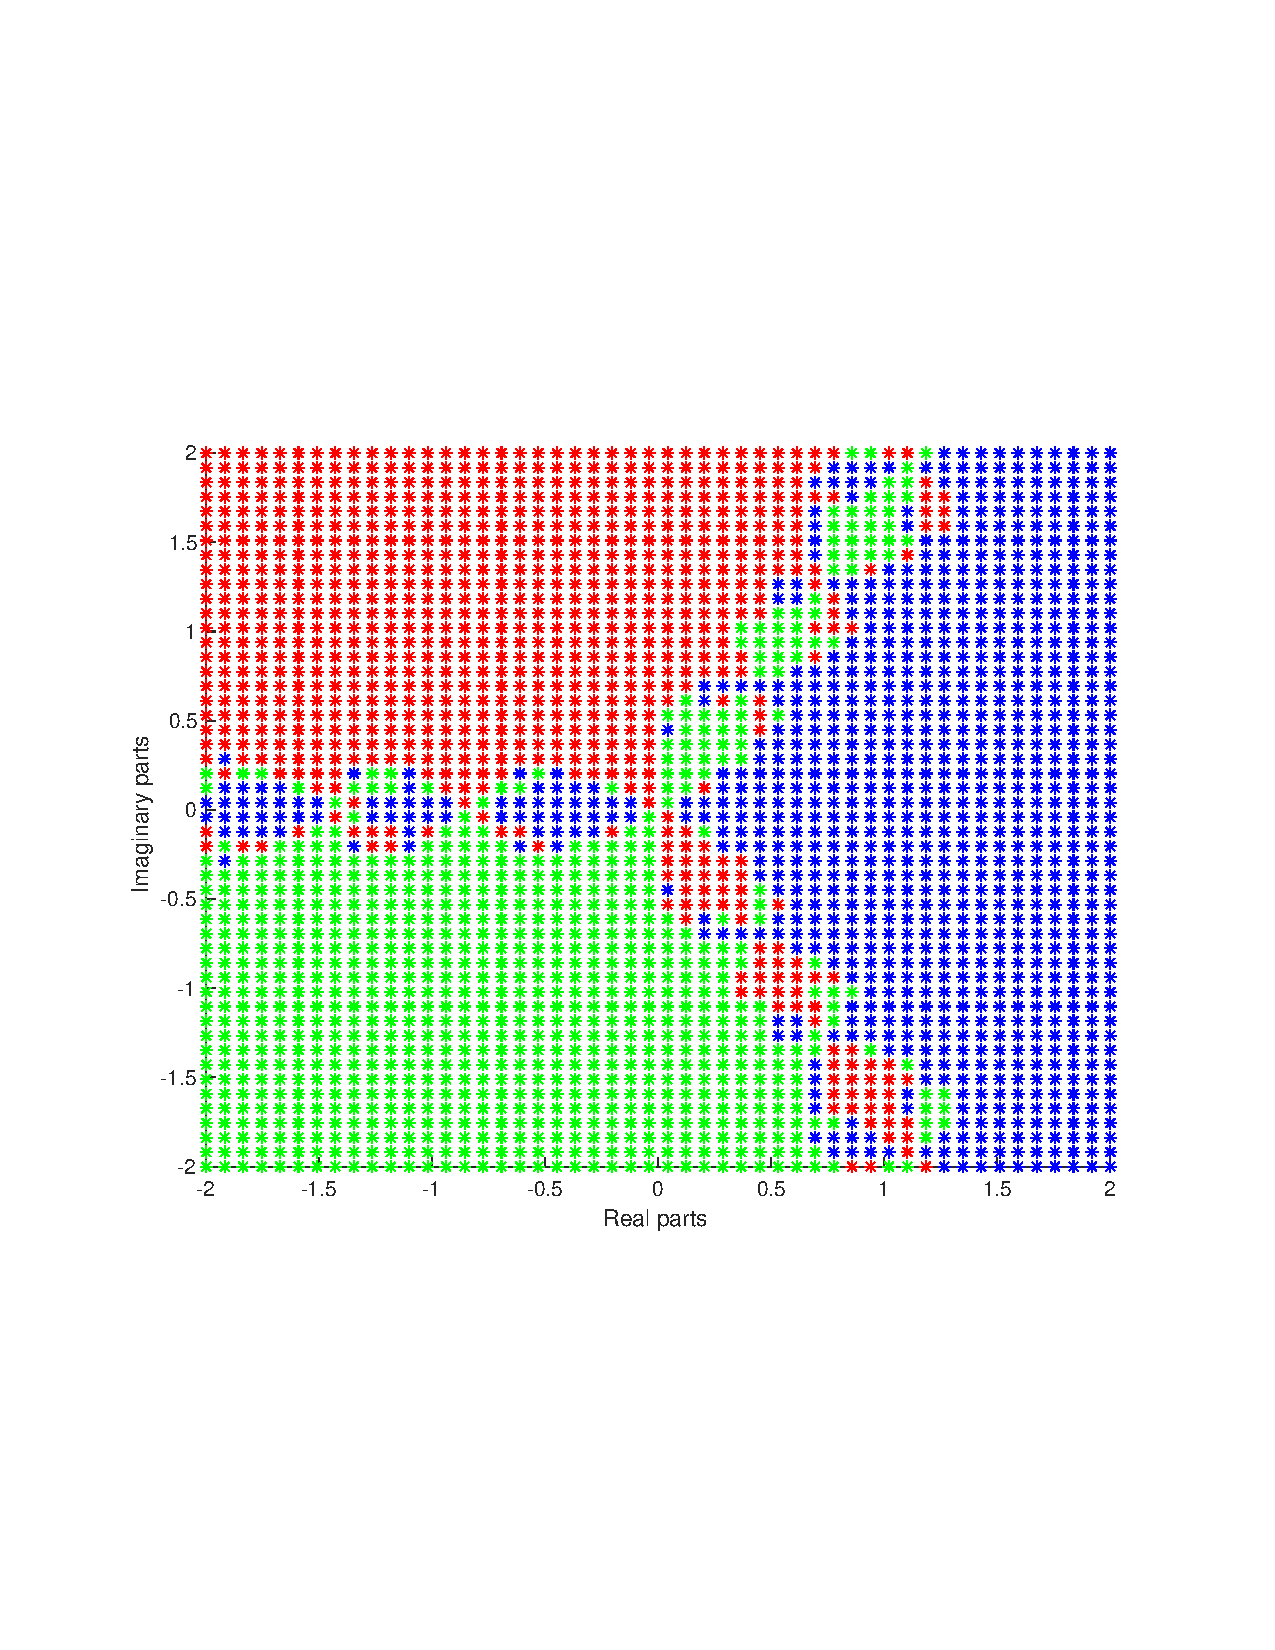
\includepdf[width=8in]{fig2.pdf}

     \subsection{Applying Newton's Method for 'Part c'}
   The task is to make a selection of pictures zooming in so the figure has more detail, and verify that the detail continues as you zoom in – it is a fractal. This is accomplished in lines 59 to 111 of 'Project2.m'.\par
   
   \begin{figure}[ht!]
    \centering
    \begin{subfigure}{0.35\textwidth}
        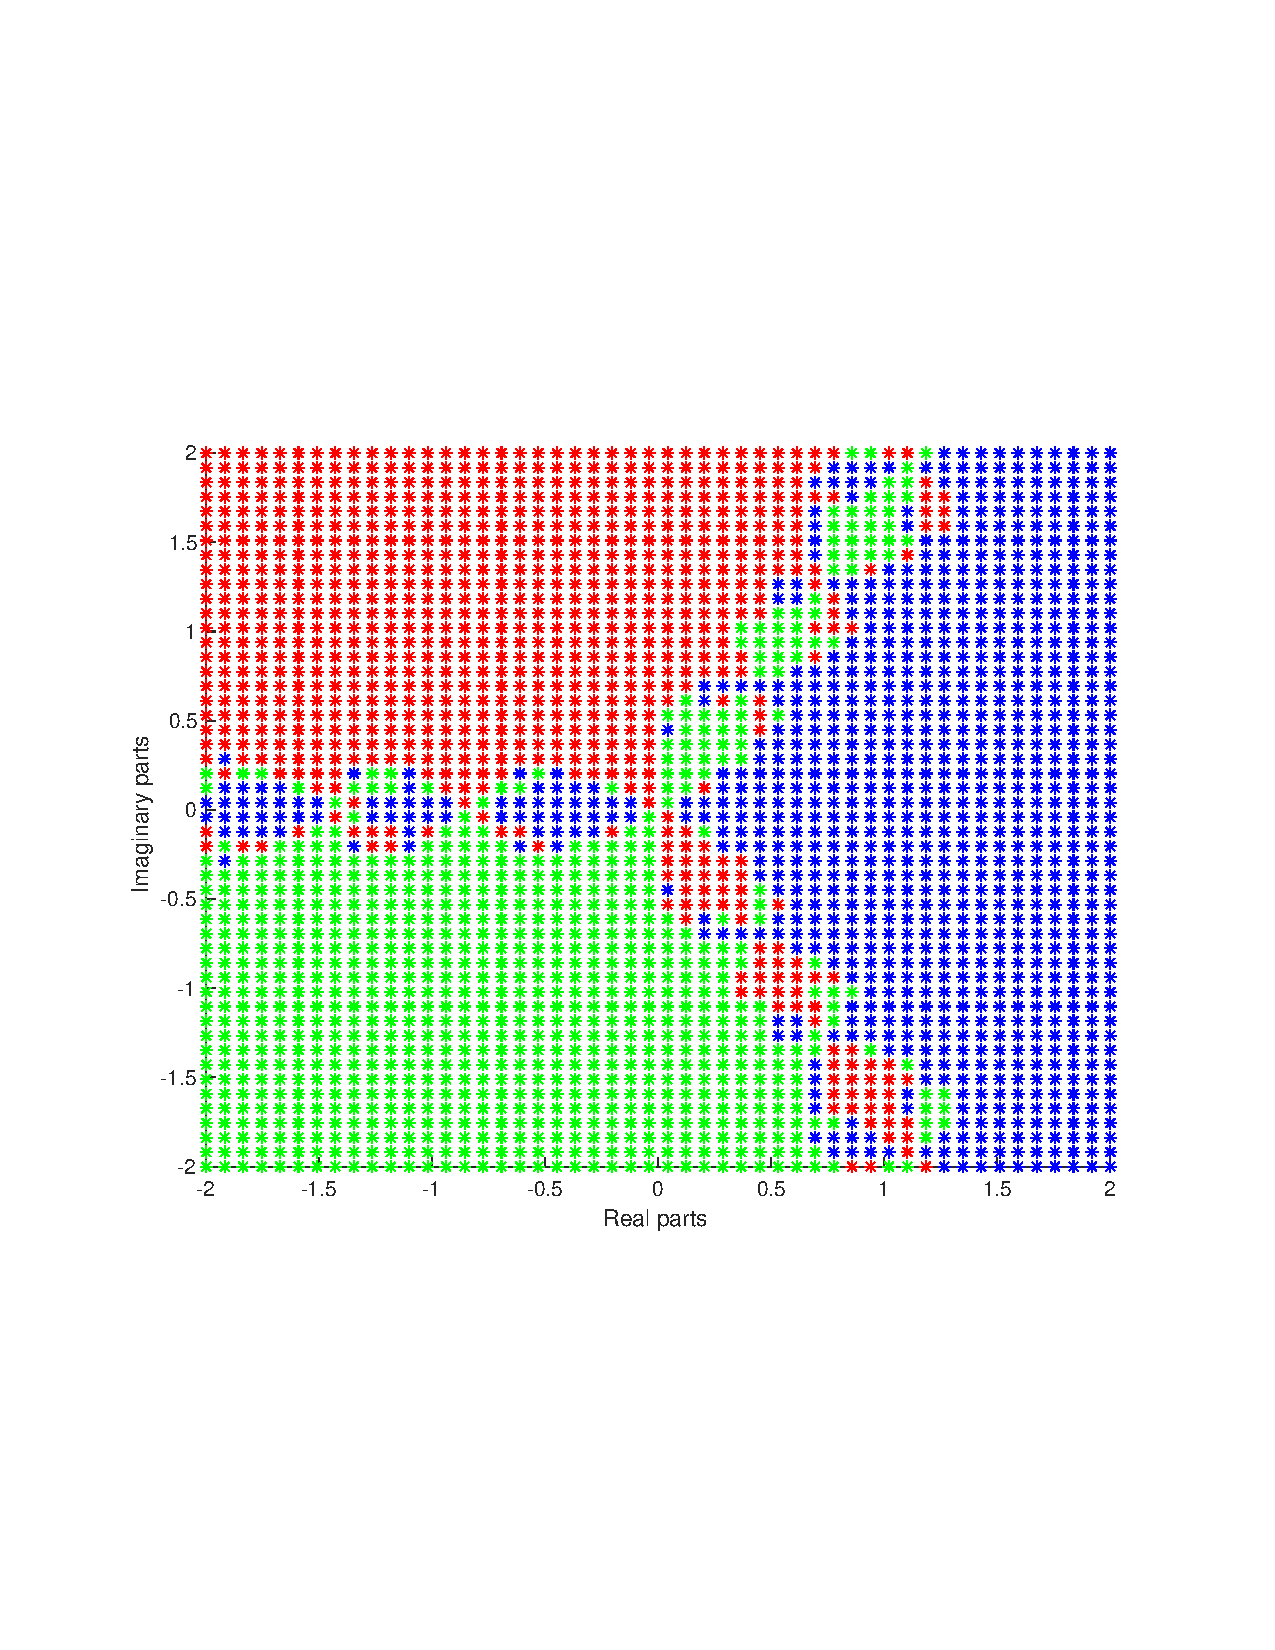
\includegraphics[width=\textwidth]{fig2.pdf}
        \caption{\small}
        \label{}
    \end{subfigure}
    \begin{subfigure}{0.35\textwidth}
        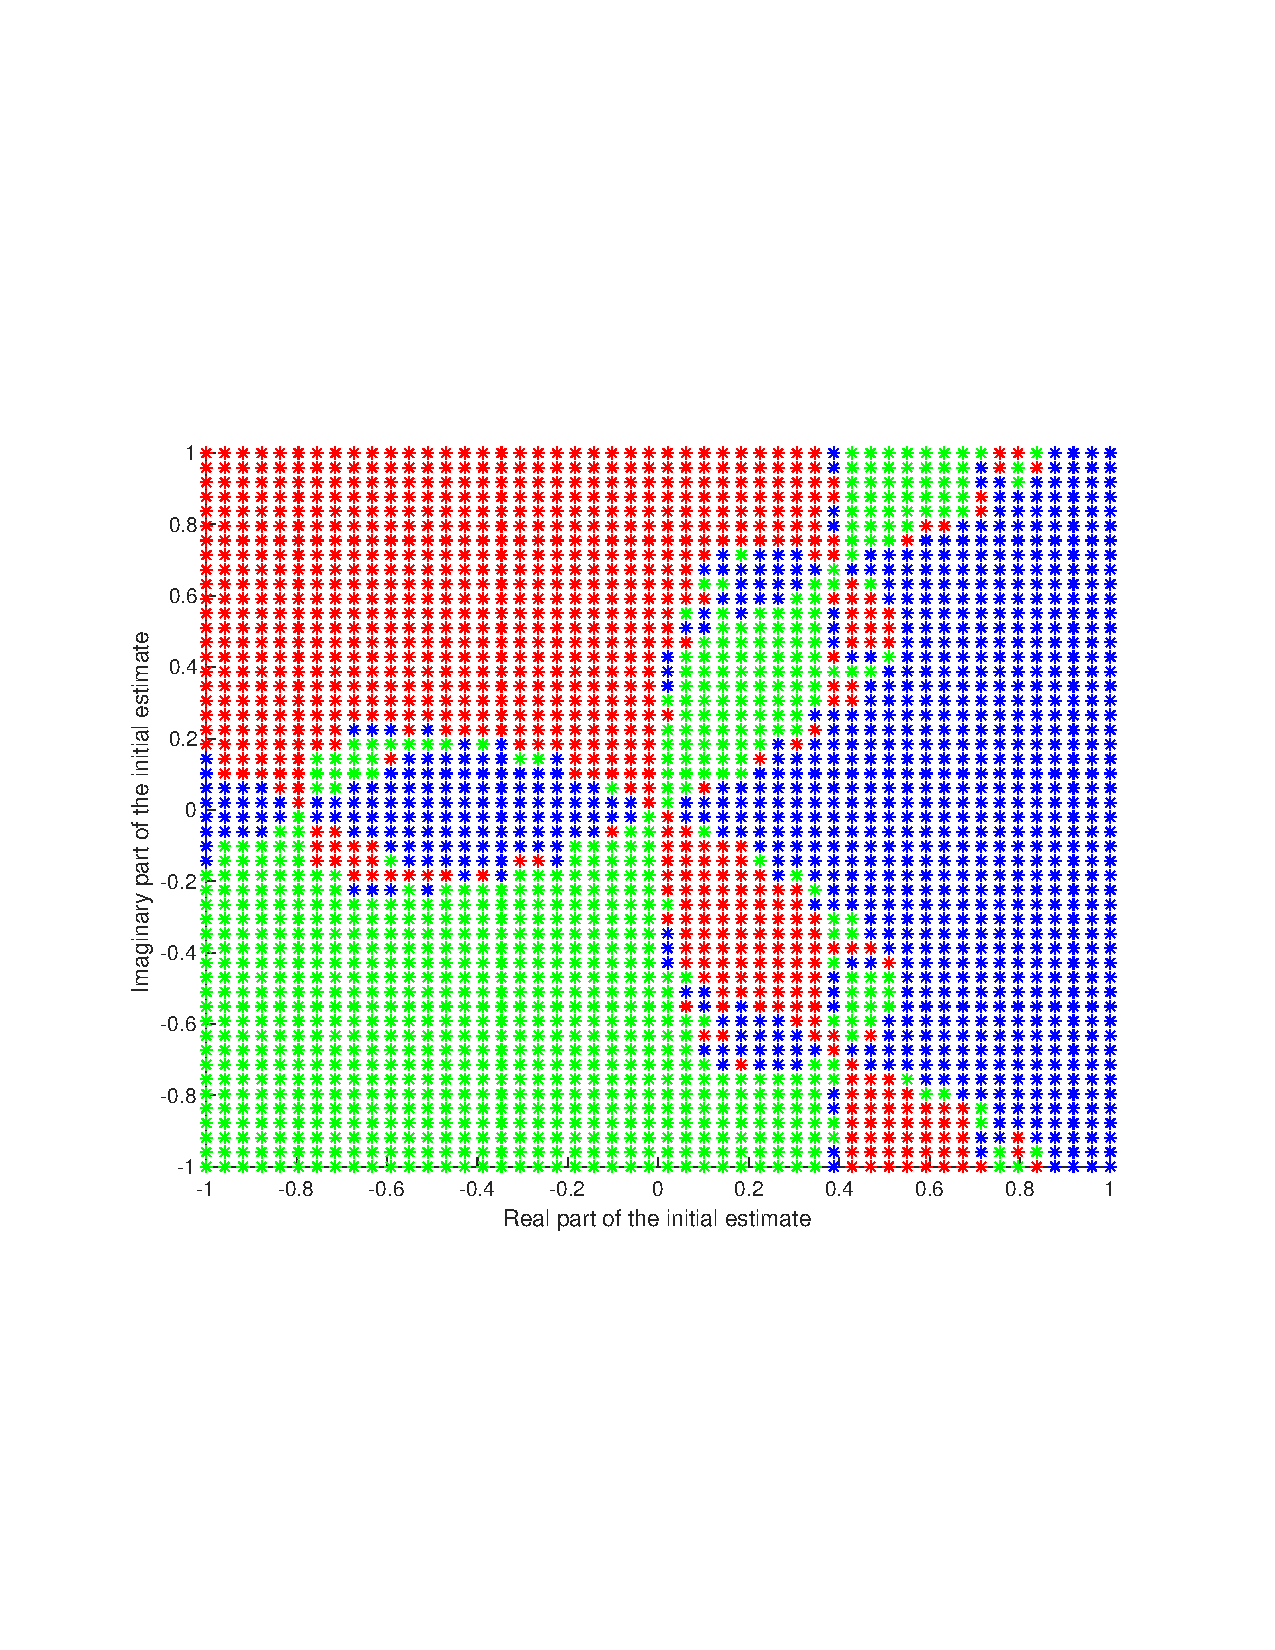
\includegraphics[width=\textwidth]{fig3.pdf}
        \caption{\small }
        \label{}
    \end{subfigure}
    \begin{subfigure}{0.35\textwidth}
        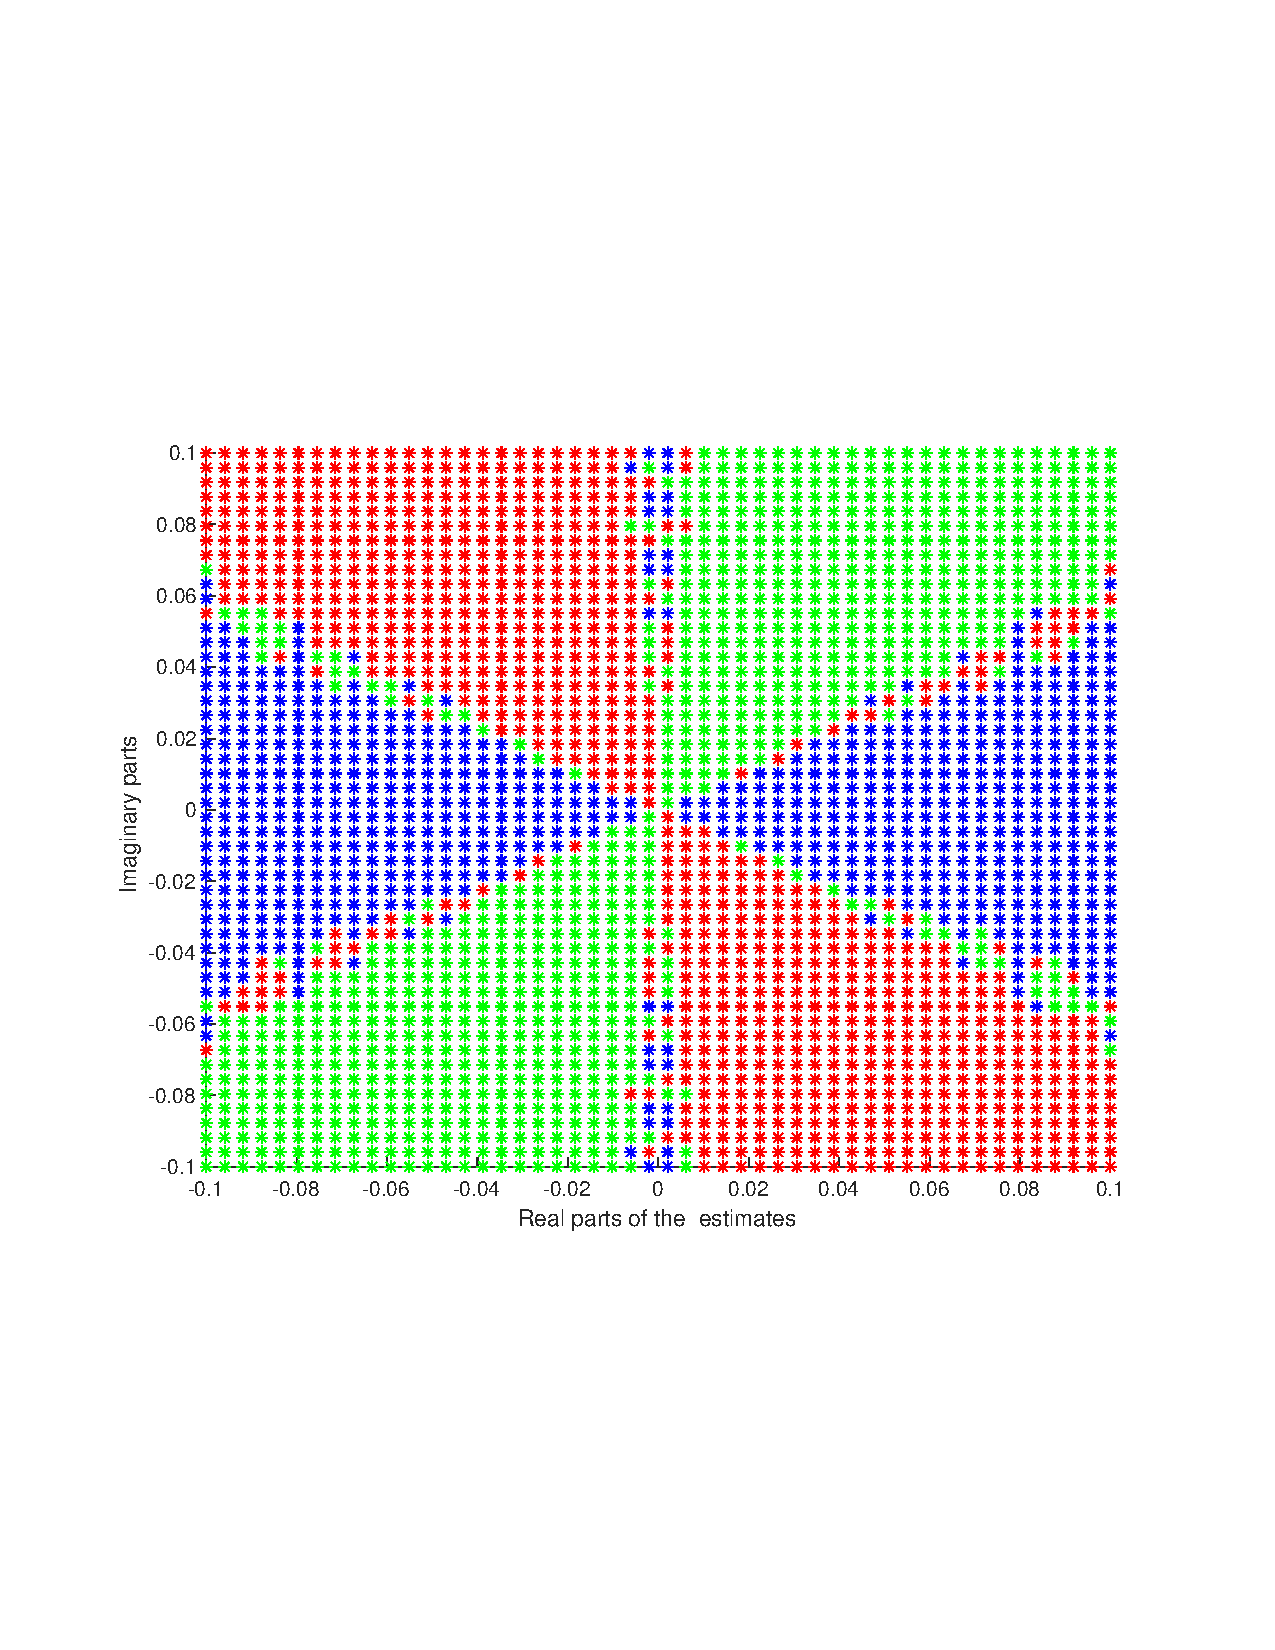
\includegraphics[width=\textwidth]{fig4.pdf}
        \caption{\small }
        \label{}
    \end{subfigure}
\end{figure}
\hfill\newpage
\section{Matlab Code}
  
\lstset{language=Matlab,%
    %basicstyle=\color{red},
    breaklines=true,%
    morekeywords={matlab2tikz},
    keywordstyle=\color{blue},%
    morekeywords=[2]{1}, keywordstyle=[2]{\color{black}},
    identifierstyle=\color{black},%
    stringstyle=\color{mylilas},
    commentstyle=\color{mygreen},%
    showstringspaces=false,%without this there will be a symbol in the places where there is a space
    numbers=left,%
    numberstyle={\tiny \color{black}},% size of the numbers
    numbersep=9pt, % this defines how far the numbers are from the text
    emph=[1]{for,end,break},emphstyle=[1]\color{red}, %some words to emphasise
    %emph=[2]{word1,word2}, emphstyle=[2]{style},    
}
\lstinputlisting{AChaoticNewton.m}
\subsection{AChaoticNewton.m}
\lstinputlisting{AChaoticNewton.m}
\hfill\newpage
\subsection{Project2.m}
\lstinputlisting{Project2.m}

\section{Discussion of results and conclusions}
  \subsection{Results}
  The results of this analysis is Equation (2) is what we define to be a 'fractal' - a complex geometric shape commonly exemplifying fractional dimensions.  
  \subsection{Conclusions}
  These algorithms work properly: Project2.m uses the AChaoticsNewton function to find the roots of Equation (1) as well as Equation (2).  The imaginary and real parts for Equation (2) form a fractal illustrated in Subsection 1.3.

\end{document}